\documentclass[../rapport_MVEX01-11-05]{subfiles}
\begin{document}

\subsection{$k$-nearest-neighbour}\label{sec:knn}

\knn eller $k$ närmsta grannar är en klassificeringsmetod som baserat
på
prototypobjekt i egenskapsrummet tilldelar en klass till en observerad
punkt i rummet.
Prototypobjekten är redan klassificerade objekt i en inlärningsmängd,
och uppgiften är att bestämma vilken klass ett nytt testobjekt tillhör.

Klasserna är här olika statiska gester, eller olika grupper i
egenskapsrummet. För
varje observerad bildruta undersöker man alltså vilken klass den tillhör.

Avståndet som används är det euklidiska, dvs
\begin{equation*}
    d = \left(\sum_{i=1}^n(\vect{x}_i-\vect{x_0}_i)^2\right)^{1/2}
\end{equation*}
där $n$ är dimensionen på egenskapsrummet, $\vect{x}$ är koordinaterna för en
prototyp och $\vect{x_0}$ är observationen. Genom en uttömmande sökning i
featurerummet letar vi efter de $k$ närmsta grannarna. Om $k$ är större än ett
avgörs klasstillhörigheten genom majoritetsomröstning, dvs. den klass med flest
nära grannar vinner, se figur \ref{fig:knn-overview}.

\begin{figure}[!htb]
    \begin{center}
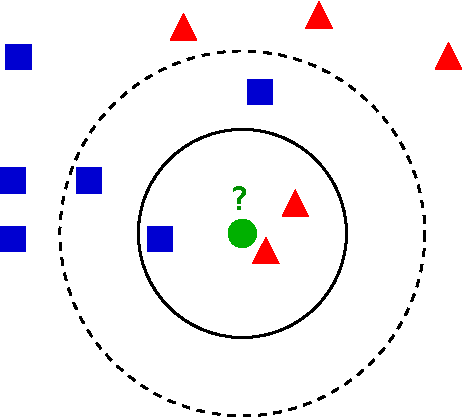
\includegraphics[width=0.75\textwidth]{bilder/KnnClassification}
    \end{center}
    \caption{kNN-klassificering av den runda observationen i mitten i ett rum
    med två klasser, trianglar och kvadrater. Majoritetsomröstning
    med $k=3$ leder till att den runda klassas som triangel, medan $k=5$ leder
    till klassificering som kvadrat.}
    \label{fig:knn-overview}
\end{figure}

För att metoden ska fungera krävs att alla klasser är representerade med lika
många prototypobjekt, annars får vissa klasser större vikt och kommer med högre
sannolikhet att väljas. Metoden bygger också på att en stor mängd data finns
tillgänglig --- prototypmängden representerar då den sanna
fördelningen hos datamängden
och är därför ofta att föredra framför en Gaussian Mixture Model, där
varje klass
approximeras av sina anpassade parametrar.
\notes{cite Röding?}

%Detta måste givetvis göras en gång per gest, vilket ger oss en kodbok
%per gest; detta eftersom vi har en HMM per gest.
%
%\marginpar{Eller, hur ska vi göra egentligen? En eller flera
% kodböcker? Hur skalar algoritmerna, hur jobbigt blir det? Säger
% någon referens något om detta?}

%FIGUR
%http://en.wikipedia.org/wiki/File:KnnClassification.svg

\end{document}
